\textbf{An introduction to peeragogical asssessment}

\subsubsection{Different ways to analyze the learning process}

After doing some personal reflection on the roles you want to take on
and the contributions you want to make (as we discussed above), you may
also want to work together with your learning group to analyze the
learning process in more detail. There are many different phases,
stages, and dimensions that you can use to help structure and understand
the learning experience: we list some of these below.

\begin{enumerate}
\item
  I, We, Its, It (from Ken Wilber -- for an application in modeling
  educational systems, see {[}1{]})
\item
  Guidance \& Support, Communication \& Collaboration, Reflection \&
  Demonstration, Content \& Activities (from Gráinne Conole)
\item
  Forming, Norming, Storming, Performing from Bruce Tuckman.
\item
  The ``five-stage e-moderating model'' from Gilly Salmon
\item
  Assimilative, Information Processing, Communicative, Productive,
  Experiential, Adaptive (from Oliver and Conole)
\item
  Multiple intelligences (after Howard Gardner).
\item
  The associated ``mental state'' (after Csíkszentmihályi; see picture)
\item
  Considered in terms of ``Learning Power'' (Deakin-Crick, Broadfoot,
  and Claxton).
\end{enumerate}

\begin{figure}
\begin{center}
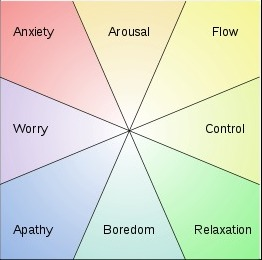
\includegraphics[width=.6\textwidth]{../pictures/challenge.jpg}
\end{center}
\caption*{
 \href{http://commons.wikimedia.org/wiki/File\%3AChallenge\_vs\_skill.svg}{Challenge
 vs. Skill}. By w:User:Oliverbeatson (w:File:Challenge vs skill.jpg)
{[}Public domain{]}}
\end{figure}

\subsubsection{Peer learning for one}

How can you apply the ideas of peer learning on your own? In a certain
sense, it's impossible, but somehow that never stops people from trying.
We find a striking parallel between the paragogy principles and the 5
Elements of Effective Thinking proposed by Edward Burger and Michael
Starbird in a recent book {[}2{]}. It's a nice short book and worth a
read: here, we will just quote the titles of the main chapters to
illustrate one possible parallel:

\begin{enumerate}
\item
  Changing context as a decentered center \ensuremath{\sim}
  Quintessence, Engaging Change: Transform Yourself
\item
  Meta-learning as a font of knowledge \ensuremath{\sim} Earth,
  Grounding Your Thinking: Understanding Deeply
\item
  Peers provide feedback that wouldn't be there otherwise
  \ensuremath{\sim} Air, Creating Questions out of Thin Air: Be your own
  Socrates
\item
  Learning is distributed and nonlinear \ensuremath{\sim} Water, Seeing
  the Flow of Ideas: Look Back, Look Forward
\item
  Realize the dream if you can, then wake up! \ensuremath{\sim} Fire,
  Igniting Insights through Mistakes: Fail to Succeed
\end{enumerate}
We think that ``thinking'' is often most effective when it's done with
others, and this is something that Burger and Starbird don't give much
attention. Nevertheless, even when you find yourself on your own in the
midst of that challenging DIY project, you can use the techniques of
peer learning to understand yourself as a growing, changing part of a
shared context in motion. This can contribute to an effective and
adaptive outlook on life.

We invite you to approach this book as a ``peer learner'' -- and we hope
the techniques we've introduced here will serve you well in the world at
large. The section on
\href{http://peeragogy.org/assessment/}{peeragogical assessment} will
help you further hone your critical peer learning edge.

\subsection{References}

\begin{enumerate}
\item
  Corneli, J., and Mikroyannidis, A. (2012). Crowdsourcing education on
  the Web: a role-based analysis of online learning communities, in
  Alexandra Okada, Teresa Conolly, and Peter Scott (eds.), Collaborative
  Learning 2.0: Open Educational Resources, IGI Global.
\item
  Burger, E. and Starbird, M. (2013). The 5 Elements of Effective
  Thinking, Princeton University Press.
\end{enumerate}
